\documentclass[11pt,a4paper]{article}
\usepackage[utf8]{inputenc}
\usepackage[french,frenchb,francais]{babel}
\usepackage[T1]{fontenc}
\usepackage{amsmath}
\usepackage{amsfonts}
\usepackage{amssymb}
\usepackage{graphicx}
\usepackage{hyperref}
\hypersetup{%
 pdfborder = {0 0 0}
}
\author{\textsc{\textbf{Phélipot Pascal}}\\\textsc{Noro Geoffrey}\\\textsc{Ralijaona Tiona}\\\textsc{Rimoux Quentin}}
\title{Projet de BDD : Gestion au Moyen Age}
\date\today

\begin{document}
\pagenumbering{gobble}
\maketitle
\pagestyle{plain}
\newpage
\tableofcontents

\newpage\pagenumbering{arabic}
\section{Introduction}
\subsection{L'idée}
Le projet est un jeu par navigateur orienté stratégie en multijoueur. 
Chaque joueur dispose d'une base sur une carte. Il a la possibilité d'y construire des bâtiments, de gérer ses ressources et de lancer la recherche de nouvelles technologies.
Les ressources sont générées chaque minute pour chaque utilisateur et il faut améliorer ses bâtiments pour en produire plus. \\
Le but du jeu est d'attaquer les autres joueurs afin de gagner des ressources et d'améliorer sa base au maximum. \\


\subsection{Répartition des rôles}
\subsection{Mise en œuvre}
\begin{itemize}
	\item Carte du monde 
	La carte a été faite par Quentin.
	\item Moteur du jeu \\
	La création du moteur du jeu a été attribuée à Pascal. Il doit réaliser la gestion des tours.
	\item Affichage
	Geoffrey et Tiona ont été chargé de l'affichage et la gestion des différents modèles. 
	\item Données \\
	Tout le monde a participé à l'ajout de nouvelles unités et de bâtiments.
\end{itemize}
\subsection{Gestion de projet}
Pour gérer ce projet nous avons bosser tout ensemble simultanément grâce à la plate-forme Github, qui permet de gérer la version de son code et de fusionner les travaux de chacun.\\
Le projet est accessible en ligne à l'adresse :  \url{http://www.github.com/pasterp/GestionMiddleAge}

\newpage\section{Représentation des données}
\subsection{Modèle-Vue-Contrôleur}
Pour concevoir notre projet, nous avons souhaité nous orienter vers une organisation de notre code en MVC ( Modèle-Vue-Contrôleur) avec du PHP orienté objet. Ce système nous a permis de bien structurer notre code. Nous avons donc créer 3 répertoires permettant de rangés les fichiers modèles, vues et contrôleurs de chacune des tables principales. En ce qui concerne les tables de jonctions quand à elle ne sont présentes uniquement dans des fonctions introduites dans les modèles des autres tables.
\subsection{Base de Données}
(Voir Annexes Page I) \\
La base de données contient les joueurs, les cases de la carte, les différents bâtiments, les ressources et les unités.  \\
Tous les liens entres ces différentes entités sont dans des tables de jointures.\\
Une table est également utilisé pour la gestion du temps.

\newpage\section{Gestion des tours}
Pour gérer les actions des joueurs, on a besoin de la notion du temps. Il faut donc que notre site opère certaines opérations au fil du temps. \\
Il va devoir attendre une certaine durée (qu'on appellera cycle) qui a été définie à 15 minutes et ensuite lancer des actions telles que la génération des ressources, l'avancée d'une armée, etc...\\
\subsection{Les possibilités}
\subsubsection{Ajax}
L'AJAX (Asynchronous JavaScript and XML) est un outil permettant via un Javascript de modifier la structure d'une page en direct. 
Ce dernier peut donc appeler les fonctions désirées quand un utilisateur est présent sur une page.\\
L'avantage de cette méthode est qu'elle est transparente à l'utilisateur et qu'elle permet de faire des modifications dynamiques sur la page qu'il a devant lui. \\
L'inconvénient est qu'il est nécessaire d'inclure un fichier supplémentaire et que les appels seront très concentrés sur le serveur lors de l'utilisation par un grand nombre d'utilisateur.\\
\subsubsection{Tache cron}
La tâche Cron est un système au niveau système qui permet de lancer un script à des dates et heures précises. Néanmoins Cette fonctionnalité demande des droits spécifiques au système et ne peut donc être mise en oeuvre à l'IUT. Cette méthode aurait perdu de faire un appel minimum aux fonctions (juste aux horaires désirés);
\subsection{Mise en œuvre}
La solution retenue est hybride : elle est codée en PHP mais est appelée par l'utilisateur. \\
Chaque page chargée entraîne une vérification de l'heure du dernier cycle(via mySQL), PHP compare ensuite si ce cycle est assez ancien pour faire un nouveau cycle (900 secondes dans notre code) et si c'est le cas il lance les fonctions de génération de ressources.

\newpage\section{Possibilités d'améliorations}
De nombreuses fonctionnalités de ce genre de jeu n'ont pas été implémenté et sont des possibles voies d'amélioration :\\
\begin{itemize}
\item Carte plus avancée
\item Construction de bâtiments / Entraînement d'unités
\item Gestion des combats entre utilisateurs
\item Classement des joueurs
\end{itemize}
\section{Conclusion}
\subsection{Avis personnels}
\subsubsection{Noro Geoffrey}
Lors de ce projet nous avons beaucoup travailler en équipe malgré une gestion assez mauvaise du projet qu'il faudra certainement que l'on revoit pour nos prochain projet en commun, mais l'utilisation de Github nous à facilité sa réalisation car cela nous permettait de toujours avoir une version à jour du projet et de pouvoir mettre en commun chacune de nos avancés lors de nos travaux individuel. Je penses que la chose la plus importante à revoir est donc notre gestion du temps.
\subsubsection{Phélipot Pascal}
Ce projet était peut être un peu trop ambitieux pour la durée qui nous a été donné. On a du faire preuve de beaucoup d'organisation face à sa complexité. Le manque de temps et la charge de travail des autres matières aura retardé ce projet malheureusement. Nous avons pu expérimenter le modèle MVC en PHP, bien que nous ne soyons pas sûr si notre méthode a été la bonne cela a permit une meilleure organisation.
\subsubsection{Ralijaona Tiona}
Un bon projet en perspective et de belle promesse sur papier cependant notre manque de gestion de temps et d'organisation nous a pas permis de finaliser le projet dans les temps. En effet, je reste sur ma faim et me dis que j'aurais pu aboutir le projet. Après je retiens beaucoup de positif, car j'ai pu découvrir la programmation orientée objet en PHP et travailler sur le modèle MVC ( Modèle Contrôleur Vue) afin d'avoir une meilleur organisation dans les fichiers. 
\subsubsection{Rimoux Quentin}
Ce projet m'a permis de mieux cerner les difficultés de gestion et de réalisation que l'on peut rencontrer en groupe. De plus, il m'a fait réaliser qu'avoir de l'ambition peut parfois être une mauvaise chose. En revanche, ce projet m'a permis de mieux appréhender l'implémentation d'une base de données avec un site Web et m'a fait découvrir la programmation orienté objet en PHP ainsi que l'utilisation du modèle MVC en Web.
\subsection{Avis Global}
Le temps a manqué pour ce projet vis à vis de nos ambitions. Nous avons néanmoins réussi à fournir de nombreuses fonctionnalités comme nous le voulions: gestion des utilisateurs, gestion du temps et des ressources.\\
Nous avons également appris à mieux nous organiser et le prochain projet devrait être plus simple à mettre en place.

\newpage\pagenumbering{Roman}
\section{Annexes}
\subsection{Base de données}
\subsubsection{MySql prévu}
\begin{figure}[!h]
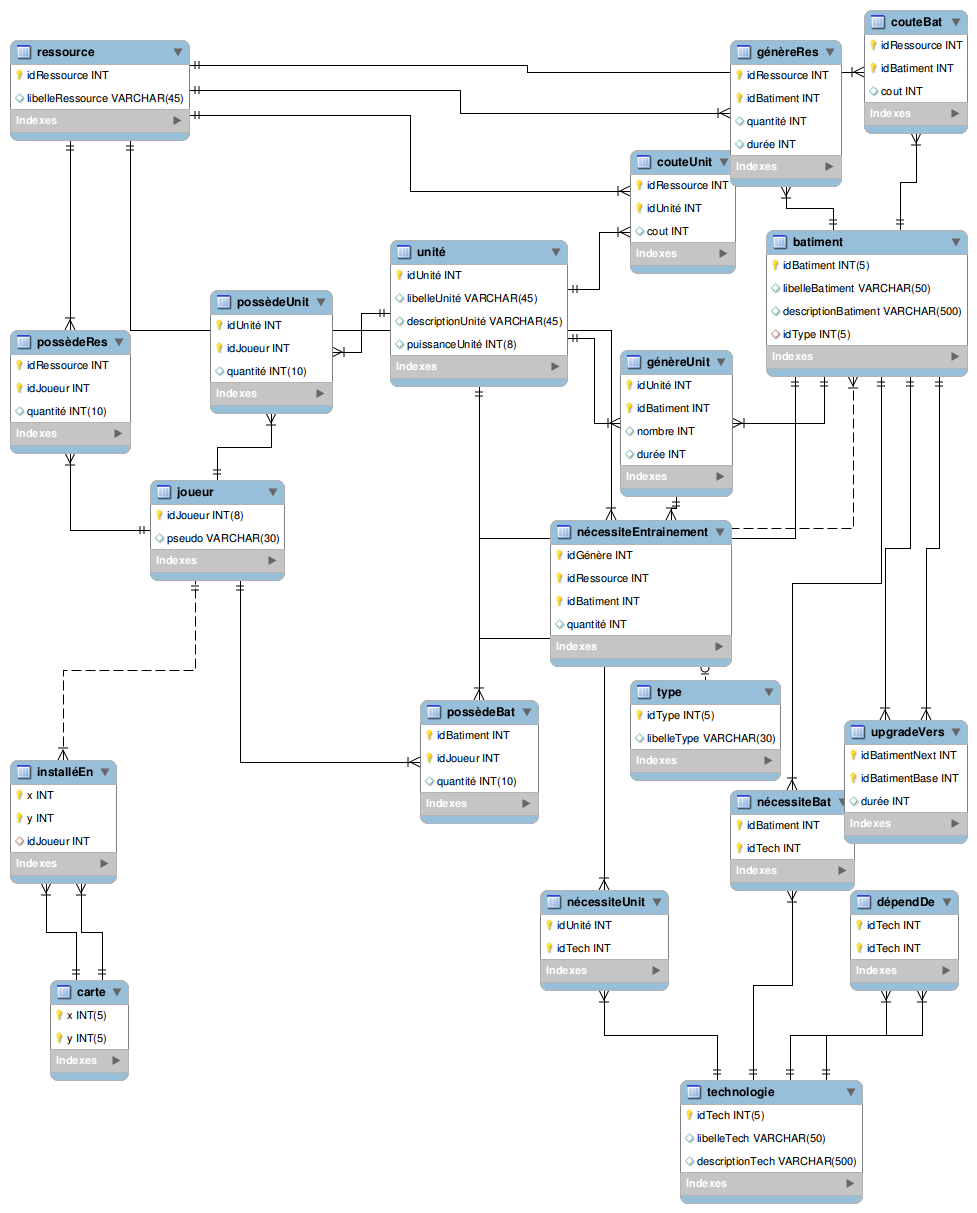
\includegraphics[scale=0.3]{./sql/last.png}
\end{figure}
\newpage\subsubsection{MySql final}
\begin{figure}[!h]
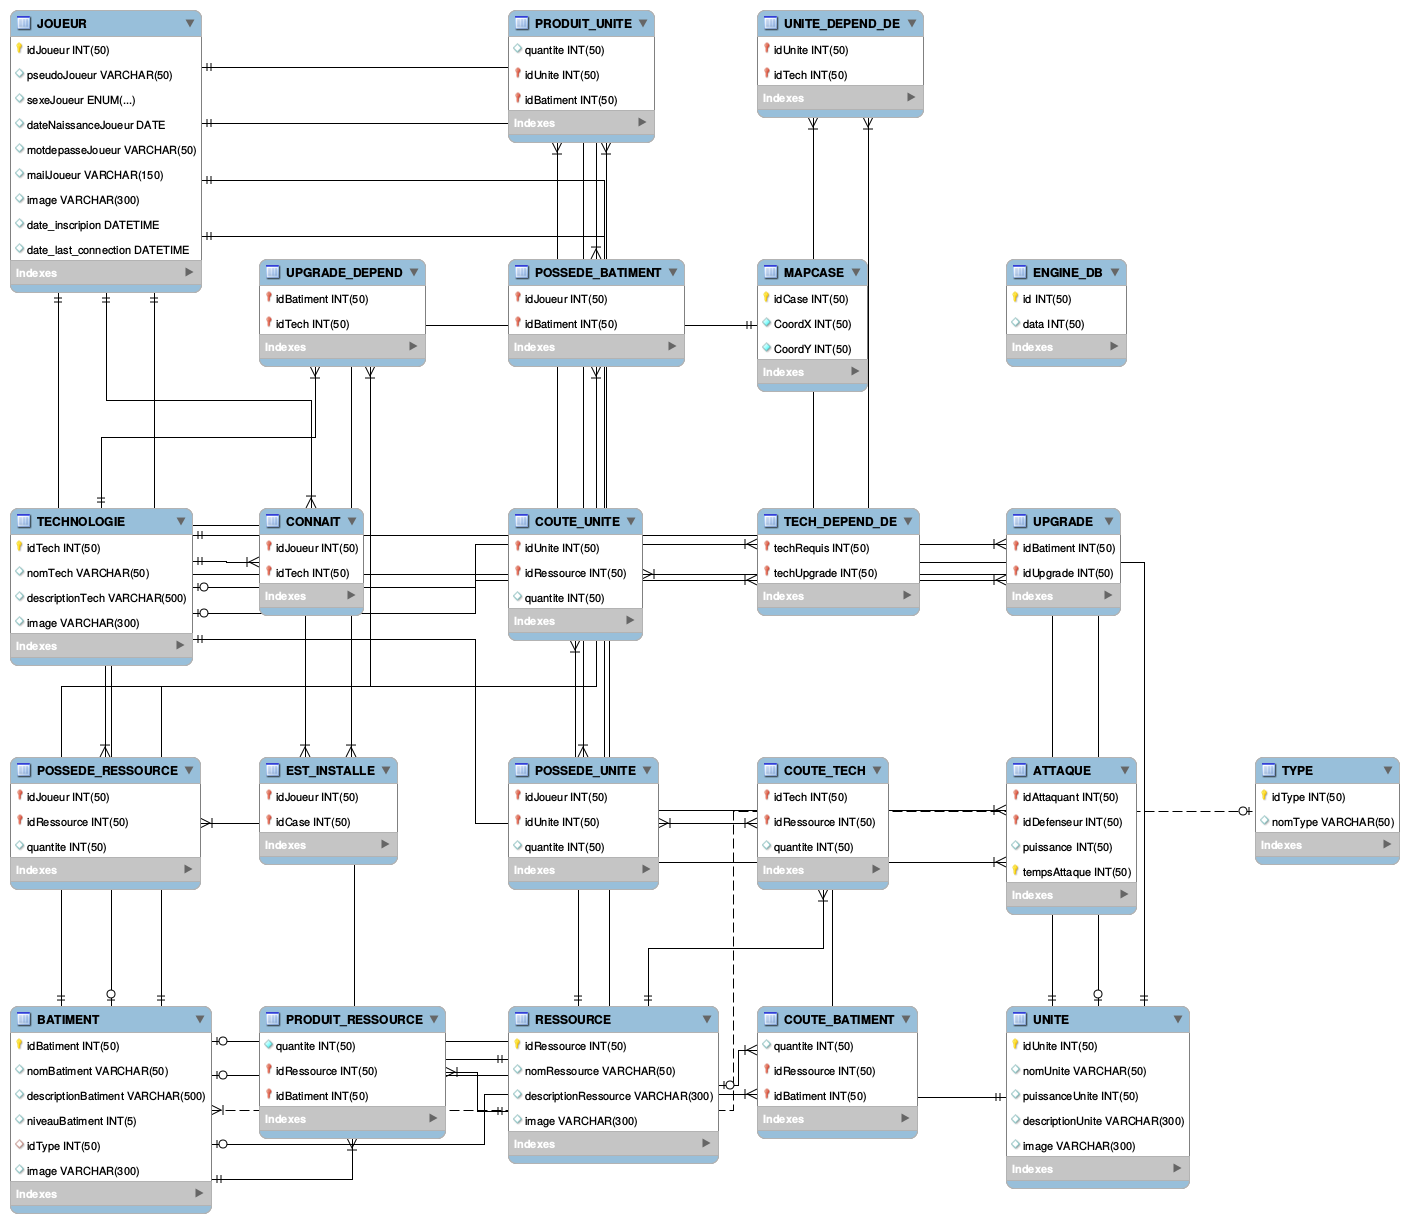
\includegraphics[scale=0.3]{./sql/final.png}
\end{figure}
\end{document}